\documentclass[11pt,a4paper]{article}

\usepackage[utf8]{inputenc}
\usepackage[margin=1in]{geometry}
\usepackage{booktabs}
\usepackage{graphicx}
\usepackage{amsmath}
\usepackage{listings}
\usepackage{xcolor}
\usepackage{float}
\usepackage{multirow} % FIX: required for multirow tables

% Optional (recommended for better number alignment)
% \usepackage{siunitx}

% Code listing configuration
\definecolor{codegreen}{rgb}{0,0.6,0}
\definecolor{codegray}{rgb}{0.5,0.5,0.5}
\definecolor{codepurple}{rgb}{0.58,0,0.82}

\lstset{
    language=Verilog,
    basicstyle=\ttfamily\small,
    keywordstyle=\color{blue},
    commentstyle=\color{codegreen},
    stringstyle=\color{codepurple},
    breaklines=true,
    frame=single,
    showstringspaces=false
}

\title{Experiment Report: Pipelined FIR Filter Implementation and Resource Analysis}
\author{EE24BTECH11048\\NITHIN K}
\date{March 25, 2026}

\begin{document}

\maketitle

\section{Introduction}
This report evaluates the performance and hardware resource utilization of Finite Impulse Response (FIR) filters implemented on the Intel Cyclone V FPGA (5CEBA2F17A7). We compare non-pipelined and pipelined architectures across three implementation methodologies: Direct, Optimized, and Genvar-based.

\section{Pipelined Architecture Explanations}

Pipelining increases maximum operating frequency ($F_{max}$) by inserting registers between combinational stages.

\subsection{Direct Pipelined Form}
The Direct Pipelined module (\texttt{dir\_pipe.v}) registers multiplier outputs. However, the accumulation is performed combinationally, creating a critical path in the adder tree, which limits $F_{max}$.

\subsection{Optimized Pipelined Form}
The Optimized module (\texttt{opt\_pipe.v}) pipelines both multiplication and accumulation:

\begin{equation}
stage[i] \Leftarrow stage[i-1] + ((x \cdot h[i]) \gg 14)
\end{equation}

This reduces combinational depth to a single multiplier–adder path per stage.

\subsection{Genvar Pipelined Form}
The Genvar implementation (\texttt{genvar\_pipe.v}) uses a Verilog \texttt{generate} loop to instantiate parameterized pipeline stages, enabling scalable hardware replication.


\section{Analysis of Results}

\begin{itemize}
    \item \textbf{DSP Limitation:} Direct and unoptimized designs exceed available DSP resources, causing synthesis failure.
    \item \textbf{Register Overhead:} Pipelining increases register usage due to intermediate stage storage.
    \item \textbf{Efficiency:} Optimized and Genvar pipelined designs successfully fit within device constraints while maintaining throughput.
\end{itemize}

\begin{figure}[H]
    \centering
    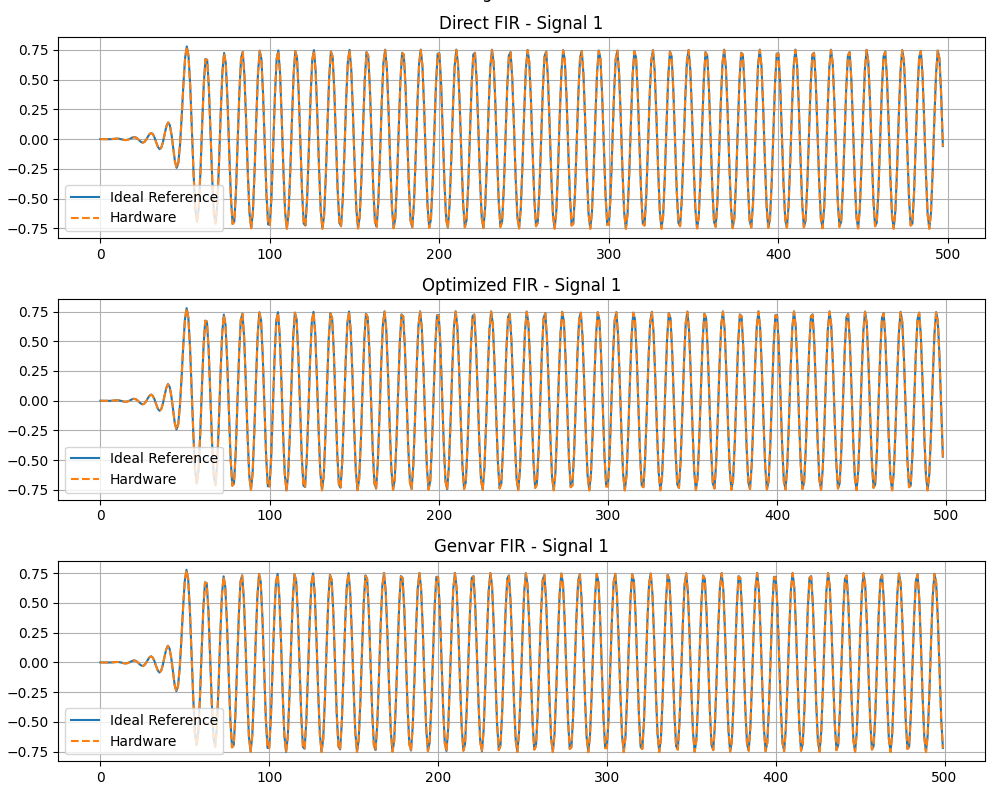
\includegraphics[width=1.0\textwidth]{signal1.png}
    \caption{Signal 1 output comparison}
\end{figure}

\begin{figure}[H]
    \centering
    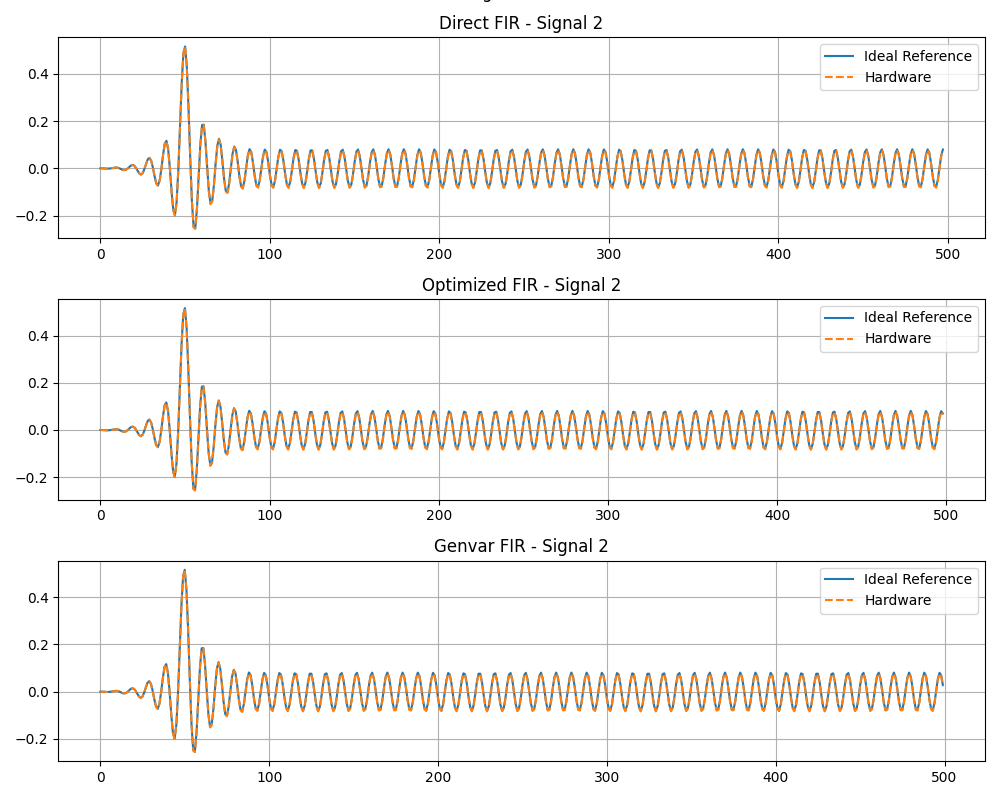
\includegraphics[width=1.0\textwidth]{signal2.png}
    \caption{Signal 2 output comparison}
\end{figure}

\begin{figure}[H]
    \centering
    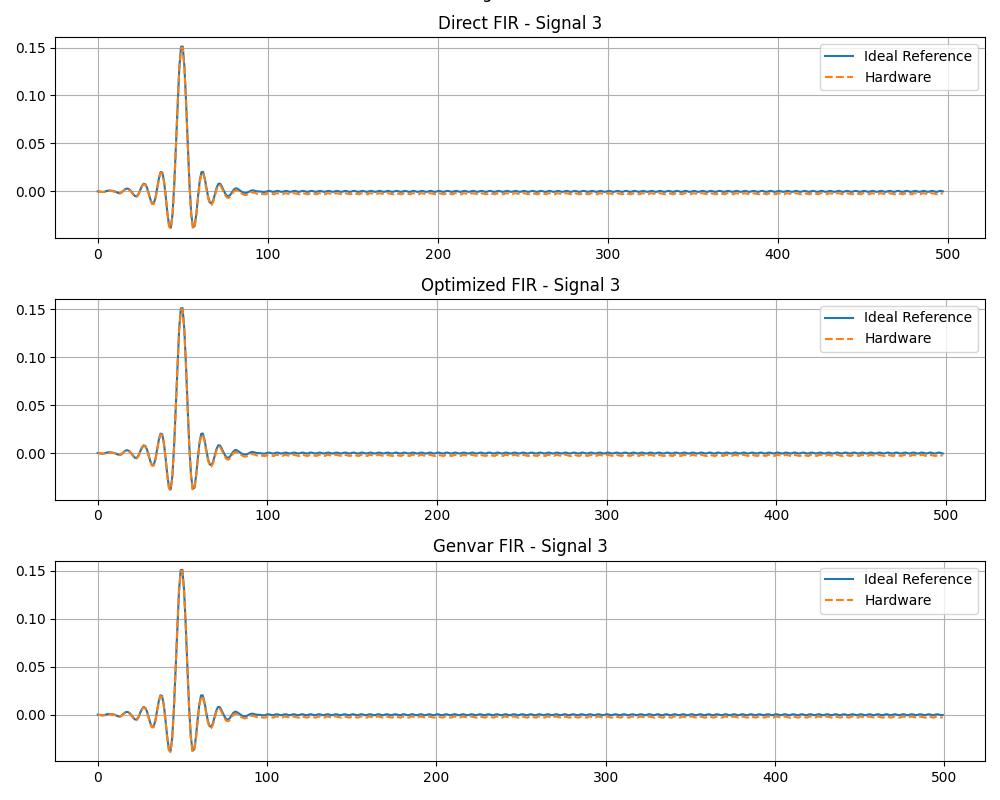
\includegraphics[width=1.0\textwidth]{signal3.png}
    \caption{Signal 3 output comparison}
\end{figure}

\section{Error Analysis and Performance Comparison}

\begin{table}[H]
\centering
\renewcommand{\arraystretch}{1.3}

\begin{tabular}{|c|c|c|c|c|}
\hline
\textbf{Signal} & \textbf{Method} & \textbf{Shift (cycles)} & \textbf{Max Error} & \textbf{Mean Error} \\
\hline

\multirow{3}{*}{Signal 1}
& Direct    & 2 & 0.0035306 & 0.0026868 \\
& Optimized & 1 & 0.0035306 & 0.0026872 \\
& Genvar    & 1 & 0.0035306 & 0.0026869 \\
\hline

\multirow{3}{*}{Signal 2}
& Direct    & 3 & 0.0032893 & 0.0026387 \\
& Optimized & 2 & 0.0032893 & 0.0026391 \\
& Genvar    & 1 & 0.0032893 & 0.0026397 \\
\hline

\multirow{3}{*}{Signal 3}
& Direct    & 3 & 0.0027478 & 0.0021957 \\
& Optimized & 2 & 0.0027478 & 0.0021961 \\
& Genvar    & 1 & 0.0027478 & 0.0021972 \\
\hline

\end{tabular}

\caption{Comparison of error metrics and pipeline shift across FIR implementations}
\end{table}

\section{Comparison: User Modules vs. Intel FIR IP}

The Intel FIR Compiler IP uses internal architectural optimizations such as pre-adders, dedicated pipeline registers, and DSP folding techniques, which are not directly exposed in RTL designs. This allows better resource utilization compared to manually written Verilog implementations.

\section{Conclusion}

Pipelining significantly improves timing closure in FIR filter implementations on FPGA devices. The optimized and genvar-based pipelined architectures achieve the best balance between DSP utilization, register overhead, and throughput, while direct architectures fail due to DSP resource exhaustion.

\end{document}
